\documentclass[a4paper,titlepage]{scrartcl}
\pagestyle{plain}
\usepackage[utf8]{inputenc}
\usepackage[T1]{fontenc}
\usepackage[german]{babel}
\usepackage{float}
\usepackage{graphicx,tabularx}
\usepackage{amsmath,amssymb,amstext}
\usepackage{enumerate}
\usepackage{units,longtable}
\usepackage{mhchem, numprint}

\numberwithin{equation}{section}

\title{Neutronendiffusion\\\normalsize 1. Überarbeitung}
\author{Genti Saliu, Jonas Müller\\Gruppe 106}
\date{Versuchstag: 10. November 2014}

\begin{document}
	\begin{titlepage}
		\maketitle
		\thispagestyle{empty}
	\end{titlepage}
	
\newpage
\pagenumbering{roman}
\tableofcontents

\newpage
\pagenumbering{arabic}

\section{Theoretische Grundlagen}

\subsection{Motivation}
Die Neutronendiffusion studiert die räumliche und zeitliche Ausbreitung von (thermischen) Neutronen in einem Medium, die den Gesetzmäßigkeiten der Diffusion von Gasen unterliegen. In der Anwendung spielt die Neutronendiffusion u.a. bei der Berechnung von Kernreaktoren eine Rolle.

\subsection{Neutronenerzeugung}
Neutronen sind ungeladene Teilchen, die neben den Protonen in den meisten Atomkernen vorkommen. Neutronen können auch außerhalb von Kernen existieren, man spricht dann von freien Neutronen. Diese freien Neutronen sind instabil und zerfallen nach einer gewissen Zeit in ein Proton, Elektron und Elektron-Antineutrino. Neutronen werden im Allgemeinen mit dem Formelzeichen $n$ bezeichnet.\\
Es gibten drei grundsätzliche Mechanismen um Neutronen freizusetzen:

\begin{enumerate}
\item \textbf{Kernspaltung}: Hierbei spalten sich schwere Kerne in meistens zwei kleinere Bruchstücke. Dabei entstehen schnelle Neutronen, zum Beispiel bei $\ce{^{235}U}$ entstehen im Schnitt 2,6 Neutronen.
\item \textbf{Kernfusion}: Zwei leichte Kerne können zu einem schwereren Kern verschmelzen. Es entstehen Neutronen und andere Strahlungsarten. Ein Beispiel ist die Verschmelzung von einem Deutron mit einem Tritiumkern, wobei $\alpha$-Teilchen und ein Neutron emittiert werden.
\item \textbf{Kernreaktion}: Zur Erzeugung von Neutronen werden meistens $\gamma$-Quanten oder $\alpha$-Teilchen absorpiert und dadurch Neutronen emittiert. Diese Reaktionen nennt man dementsprechend ($\gamma, n$)- und ($\alpha, n$)-Reaktionen. Wichtig für Reaktionen der Neutronenproduktion ist ein hoher Wirkungsquerschnitt.\\
Kernspaltung und Kernfusion sind Spezialfälle der Kernreaktion.
\end{enumerate}

\subsection{Arten freier Neutronen}
Neutronen klassifiziert man entsprechend ihrer kinetischen Energien in:
\begin{enumerate}
\item \textbf{Primärneutronen} haben noch keine Stöße gemacht und besitzen ihre ursprüngliche Energie.
\item \textbf{Sekundärneutronen} haben bereits Energie verloren.
\item \textbf{Monochromatische} Neutronen besitzen eine einheitliche (gleiche) Energie.
\item \textbf{Thermische} Neutronen haben ihre überschüssige kinetische Energie vollständig auf die Materie übergeben und befinden sich im thermischen Gleichgewicht mit ihrer Umgebung. Ihre Geschwindigkeit entspricht der wahrscheinlichsten Geschwindigkeit der Maxwell-Verteilung:
\begin{equation}
v_T=\sqrt{\frac{2kT}{m}}
\end{equation}
Ihre Energie:
\begin{equation}
E=kT
\end{equation}
\end{enumerate}

\subsection{Americium-Beryllium-Neutronenquelle}
In diesem Versuch wird zur Neutronenerzeugung eine Americium-Beryllium-Neutronenquelle (Am-Be-Quelle) benutzt. Die Neutronen entstehen dabei durch eine ($\alpha, n$)-Reaktion an $\ce{^{9}Be}$:

\begin{equation}
\ce{^{9}Be} + \alpha \rightarrow n + \ce{^{12}C} + Q
\end{equation}

$Q$ gibt dabei die Differenz der kinetischen Energie der Reaktionspartner nach und vor der Reaktion an. Der $Q$-Wert beträgt in diesem Fall $\unit[5.7]{MeV}$, er ist also positiv, was bedeutet, dass Energie frei wird. Den größten Teil dieser Energie erhalten die Neutronen, denn die Rückstoßenergie des Kohlenstoffatoms ist gering.  Die Neutronen sind polychromatisch, d.h. es entsteht ein kontinuierliches Energiespektrum (siehe Abbildung \ref{fig:spektrum}). Der Grund dafür ist, dass bereits die $\alpha$-Strahlung polychromatisch ist, welche aus einer $\ce{^{241}Am}$-Quelle kommt. Außerdem unterliegen die $\alpha$-Teilchen schon vor der Reaktion einem Energieverlust in der Quelle.\\
\begin{figure}[H]
	\centering
	\begin{tabular}{@{}r@{}}
		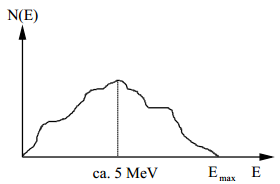
\includegraphics[width=0.4\textwidth]{images/spektrum.PNG}\\
		\footnotesize\sffamily\textbf{Quelle:} Blaues Buch \cite{blauesBuch}
	\end{tabular}
	\caption{Spektrum einer Neutronenquelle}
    \label{fig:spektrum}
\end{figure}
Die wahrscheinlichste Neutronenenergie liegt bei ungefähr $\unit[5]{MeV}$. Die maximale Energie ergibt sich aus:

\begin{equation}
E_{max}= Q + E_{\alpha}-E_{R} \approx \unit[11.19]{MeV}
\end{equation}

Man verwendet hier eine $\ce{^{241}Am}$-Quelle, da diese gegenüber anderen $\alpha$-Strahlern den Vorteil hat, dass die $\gamma$-Strahlung kleine Energiewerte aufweist. Diese sind einfach abzuschirmen.

\subsection{Wechselwirkung mit Materie}
Bei der Ausbreitung von freien Neutronen druch Materie können drei Arten von Wechselwirkungen auftreten. Die Wechselwirkung findet hauptsächlich mit den Atomkernen der Materie statt. Man bezeichnet hier die Wahrscheinlichkeit, dass es zu einer Wechselwirkung kommt als $\textbf{Wirkungsquerschnitt}$.

\begin{enumerate}
\item \textbf{Elastische Stöße}: Die Summe der kinetischen Energien der Neutronen und der Kerne sind vor und nach dem Stoß gleich. Die Neutronen geben beim Stoßen Energie an die Kerne ab, da diese ursprünglich in Ruhe waren. Außerdem wird dabei das Neutron abgelenkt. Nimmt die Neutronenenergie ab, so steigt der Wirkungsquerschnitt.
\item \textbf{Inelastische Stöße}: Im Gegensatz zu den elatischen Stößen ist hier die Summe der Energien nicht konstant, da ein Teil der Energie des Neutrons an den Kern als Anregungsenergie übertragen wird. Deshalb ist der Energieübertrag hier größer. Allerdings ist der Wirkungsquerschnitt geringer.
\item \textbf{Absorption}: Hierbei wird das Neutron vom Atomkern aufgenommen. Es entstehen $\gamma$-Quanten oder andere Teilchen. Wie bei den anderen Wechselwirkungen ist auch hier der Wirkungsquerschnitt bei geringeren Energien größer.
\end{enumerate}
\subsection{Wichtige Größen für den Neutronentransport}
\subsubsection{Neutronendichte}
Die Neutronendichte $n(\vec{r})$ erhält man aus der Gleichung

\begin{equation}
n(\vec{r})dV = \int_{\Omega}n(\vec{r},\vec{\Omega})dV d\Omega = \int_E \int_{\Omega}n(\vec{r},\vec{\Omega},E)dE dV d\Omega
\end{equation}

Der gesamte Ausdruck gibt dabei die Anzahl aller Neutronen im Volumenelement dV an.\\
$ n(\vec{r},\vec{\Omega},E)$ nennt man  differentielle Dichte. Diese stellt die Anzahl der Neutronen an der Stelle $\vec{r}$ mit Energien im Einheitsenergiebereich um die Energie E und mit Richtungen im Einheitsraum um $\vec{\Omega}$ da. Integriert man diese differentielle Dichte über alle Energien, so erhält man die Vektordichte $n(\vec{r},\vec{\Omega})$. Diese gibt die Anzahl der Neutronen im Volumenelemnt dV, welche sich in Richtung $\vec{\Omega}$ bewegen, an. Durch eine weiter Integration über die Raumwinkel erhält man schließlich die Neutronendichte $n(\vec{r})$.

\subsubsection{Neutronenfluss}

Der Neutronenfluss $\Phi (\vec{r})$ ist die Anzahl der Neutronen im Energieintervall von E bis E+dE, welche die Einheitsfläche senkrecht zu $\vec{\Omega}$ pro Zeiteinheit durchfliegen. Man erhält ihn aus

\begin{equation}
\Phi (\vec{r})= \int_E \int_{\Omega} n(\vec{r},\vec{\Omega},E) v(E) dEd\Omega
\end{equation}

$n(\vec{r},\vec{\Omega},E)$ ist wiederum die differentielle Dichte und über v(E) geht der Betrag der energieabhängigen Geschwindigkeiten der Neutronen ein. \\
Der Neutronenfluss kann auch über die mittlere Geschwindigkeit der Neutronen $\overline{v}$ bestimmt werden.

\begin{equation}
\Phi (\vec{r})= n(r)\overline{v}
\end{equation}

wobei die mittlere Geschwindigkeit $\overline{v}$ definiert ist durch

\begin{equation*}
\overline{v}= \frac{\int_E \int_{\Omega} n(\vec{r},\vec{\Omega},E) v(E) dEd\Omega}{\int_E \int_{\Omega} n(\vec{r},\vec{\Omega},E) dEd\Omega}
\end{equation*}

\subsection{Relaxationslänge}
Mit der Relaxationslänge $\lambda$ bezeichnet man die mittlere Weglänge, welche die Neutronen in der Materie zurücklegen, bevor sie getreut oder absorbiert werden. Sie wird bestimmt aus dem Kehrwert des totalen linearen Absorptionskoeffizienten $\Sigma_t$:

\begin{equation}
\lambda = \frac{1}{\Sigma_t}
\end{equation}

Dieser ergibt sich aus:

\begin{equation}
\Sigma_t = \Sigma_{el} + \sigma_{ab}= N (\sigma_{el} +\sigma_{ab})
\end{equation}

N ist hierbei die Teilchendichte und $\sigma_{el}$ bzw. $\sigma_{ab}$ der Wirkungsquerschnitt für die elastische Streuung bzw. für die Absorption.\\
Der Neutronenfluss einer punktförmige Quelle ist gegeben durch:

\begin{equation}
\Phi (r) = \frac{Q_0}{4 \pi r^2} e^{-\Sigma_t r}=\frac{Q_0}{4 \pi r^2} e^{-\frac{r}{\lambda}}
\label{eq:flussSchnell}
\end{equation}

$Q_0$ ist die Quellstärke, diese gibt die Anzahl der pro Zeiteinheit von der Quelle emittierte Neutronen an. Der Exponentialanteil beschreibt die Wahrscheinlichkeit, dass ein Neutron eine Strecke zurücklegt ohne mit Materie wechsel zu wirken. Diesem Anteil ist eine $\frac{1}{r^2}$-Abhängigkeit überlagert, welche sich aus der üblichen Intensitätsverteilung um eine punktförmige Quelle ergibt. Man erkennt also, dass die Relaxationslänge auch diejenige Länge ist, nach welcher sich der Neutronenfluss auf einen $e$-ten Teil verringert hat. es ist zu beachten, dass diese Gleichung des Neutronenflusses nur für Primärneutronen gilt.

\subsection{Diffusionslänge}
Die Diffusionslänge beschreibt das Absorptionsverhalten des Mediums, in dem sich die Neutronen ausbreiten, und ist ein Maß für die mittlere Entfernung $\overline{r}$ von der Quelle, in der ein Neutron absorbiert wird.\\ \\
Um sie zu bestimmen, macht man sich der sogenannten elementaren Diffusionstheorie zunutze, mit der man die energetische und räumliche Verteilung von Neutronen für eine gegebene Anordnung von Neutronenquelle und Materie bestimmt. Die Theorie geht von Vereinfachungen aus und liefert zeit- und energieunabhängige Lösungen, wobei nur Absorption und Streuung (Stöße) berücksichtigt werden und die Neutronenquelle als punktförmig angenommen wird. 

So reduziert sich die Boltzmann-Gleichung auf die folgende elementare Diffusionsgleichung:
\begin{equation}
\label{eq:boltzmann}
D \Delta^2 \Phi(r) - \Sigma_a \Phi(r) + S(r) = 0
\end{equation}
Für den Fluss gilt:
\begin{equation}
\label{eq:flussThermisch}
\Phi(r)=\frac{Q}{4 \pi D} \cdot \frac{e^{-\frac{r}{L}}}{r}
\end{equation}
Es wird eine neue Größe, die Diffusionslänge $L$, eingeführt:
\begin{equation*}
L=\sqrt{\frac{D}{\Sigma_a}}
\end{equation*}

wobei $D=\frac{1}{3 \Sigma_S}$ die Diffusionskonstante ist.

\section{Überlegungen zum Versuch}
\subsection{Ziel}
Bestimmung der Relaxationslänge schneller Neutronen und der Diffusionslänge thermischer Neutronen in Wasser.
\subsection{Aufbau}
\subsubsection{Allgemein}
Als Neutronenquelle wird eine Am-Be-Quelle verwendet, welche sich in einem Wassertank mit $\unit[100]{cm}$ Durchmesser und $\unit[80]{cm}$ Höhe befindet. Die Quelle kann mit einer Cd-Schale abgeschirmt werden. Gemessen wird die Zählrate mit und ohne Abschirmung. Zur Detektion wird ein radial verschiebbares $BF_3$-Zählrohr verwendet. Da bei dem Versuch von einer punktförmigen Quelle ausgegangen wird, ist es nicht sinnvoll bei Abständen kleiner als $\unit[14]{cm}$ zu messen.

\subsubsection{Funktionsweise $BF_3$-Zählrohr}
Bei dem $BF_3$-Zählrohr handelt es sich um ein Proportionalitätszählrohr, welches mit Borfluorid gefüllt ist. Wird ein Neutron eingefangen, kommt es unter Emittierung eines Alphateilchens zu folgender Reaktion:

\begin{equation}
n+^{10}B \rightarrow ^7Li^* + \alpha + \unit[2.31]{MeV}
\end{equation}

Es entsteht ein $^7Li$-Kern im angeregten Zustand, welcher dann unter $\gamma$-Zerfall in den Grundzustand übergeht. Anders als das Neutron, sind $\alpha$-Teilchen und $^7Li$-Kerne elektrisch geladen und erzeugen somit einen verwendbaren Messimpuls. Geben beide Teilche ihre komplette Energie ab (was sehr wahrscheinlich ist, aufgrund ihrere kurzen Reichweite), ergibt sich im Impulshöhenspektrum ein Peak bei einer Energie von $\unit[2.31]{MeV}$. Ein weiterer Peak wird sich bei $\unit[2.78]{MeV}$ ergeben, da mit einer geringen Wahrscheinlichkeit das Lithium, in der oben beschriebenen Reaktion, auch direkt im Grundzustand entsteht.
\subsection{Durchführung}
\subsubsection{Relaxationslänge}
Wie bereits erwähnt, gilt Gl. \ref{eq:flussSchnell} nur für Primärneutronen. Da zu erwarten ist, dass aber auch Sekundärneutronen gemessen werden, sollte ein komplizierterer Ausdruck zur Beschreibung des Neutronenflusses nötig sein. Allerdings streuen die Neutronen hauptsächlich an den Protonen der Wasserstoffatome und geben schnell große Teile ihrer kinetischen Energie ab. Da der Wirkungsquerschnitt mit sinkender Energie außerdem stark ansteigt, werden die Neutronen in einem kleinen räumlichen Bereich um den ersten Stoß thermalisiert. Darüber hinaus lässt sich mit einer Abschätzung zeigen, dass sich weniger als $\unit[10]{\%}$ der Neutronen um $\unit[3]{cm}$ von der Quelle entfernen. Um die Relaxationslänge für schnelle Neutronen in Wasser zu nähern, ist es also hinnehmbar den thermischen Fluss zu betrachten.\\
Durch Integration von Gleichung \ref{eq:flussSchnell} erhält man dann:

\begin{equation}
ln(r^2 \cdot \Phi (r))= - \frac{r}{\lambda} + const.
\end{equation}

Man sieht, dass es sich um eine Gerade handelt bei der die Steigung der reziproken Relaxationslänge entspricht. Wird nun der Fluss $\Phi(r)$ bei bekannter Länge $r$ gemessen, so lässt sich die Steigung, und somit die Relaxationslänge, mittels linearer Interpolation bestimmen.
\subsubsection{Diffusionslänge}
Auch in diesem Versuch wird die Am-Be-Quelle verwendet, die eine Quelle für schnelle Elektronen ist. Da wir in der Theorie von einer Quelle thermischer Neutronen ausgegangen sind, brauchen wir im Experiment auch eine solche, um die Diffusionslänge mittels in der Theorie aufgestellten Gleichungen zu bestimmen.\\ \\
Eine thermische Quelle lässt sich durch einen experimentellen Trick realisieren:
Zuerst wird der Fluss $\Phi_0(r)$ schneller Neutronen als Funktion des Abstandes von der Quelle gemessen. Dann wird um die Quelle eine Kugelschale aus Cadmium von $\unit[1]{mm}$ Dicke und einigen Zentimetern Durchmessen gelegt. Diese Schale dient als ''Filter'' und verhindert das Durchdringen von thermischen und langsamen Neutronen. Es wird dann eine zweite Messung durchgeführt (Neutronenfluss als Funktion vom Quellenabstand), wobei zum Fluss nur die schnellen und nicht mehr die langsamen und thermischen Neutronen beitragen.\\ \\
Durch Bilden der Differenz beider gemessenen Flüße in Abhängigkeit vom Abstand erhält man den Fluss der thermischen Neutronen und kann damit anhand der Gleichung \ref{eq:flussThermisch} die Diffusionslänge bestimmen.

\section{Auswertung}
\subsection{Verlauf des Versuchs}
\subsubsection{Aufbau}
Der Versuchsaufbau bestand aus einer Am-Be-Neutronenquelle, die sich in einem Wassertank mit $\unit[100]{cm}$ Durchmesser und $\unit[80]{cm}$ Höhe befand. Die Neutronenzählrate wurde mittels eines radial verschiebbaren $BF_3$-Zählrohrs gemessen, der auf Höhe der Strahlenquelle angebracht war. Es stand zusätzlich eine Cadmium-Schale zur Abschirmung des Zählrohrs von thermischen Neutronen zur Verfügung.

\subsubsection{Durchführung}
Laut Vorbereitung müssten im Versuch lediglich die Neutronenzählraten ohne und mit Cadmium-Abschirmung gemessen werden, um die Relaxations- und Diffusionslänge bestimmen zu können.\\ \\
Diese Größen werden mithilfe der elementaren Diffusionstheorie (siehe Vorbereitung) berechnet, die zur Näherung die Neutronenquelle als punktförmig annimmt. Ab einem Abstand von $\unit[14]{cm}$ kann man die Neutronenquelle als solche ansehen.\\ \\
Beginnend bei $\unit[14]{cm}$, wurden die Zählraten $N$ für $t=\unit[300]{s}$ ohne Cadmium-Abschirmung des Zählrohrs gemessen. Dazu bildeten wir am Computer, ausgehend vom Spektrum eines Vielkanalanalysators, die Summe (das Integral) aller Zählereignisse $N$. Dabei wurde nur ein bestimmter Kanalbereich des Spektrums betrachtet; die niederenergetischen Enden wurden nicht berücksichtigt, um elektronisches Rauschen und den Anteil von $\gamma$-Quanten aus der Quelle abzuschneiden. Berücksichtigt wurde der Kanalbereich 95 ($\unit[23.8]{keV}$) bis einschließlich 464 ($\unit[116]{keV}$). Der Bereich wurde bei der ersten Messung festgelegt und bei den übrigen Messungen verwendet.\\ \\
Wir erhöhten den Abstand Quelle-Zählrohr schrittweise (bei Abständen bis $\unit[20]{cm}$ um $\unit[0.5]{cm}$, danach um $\unit[1]{cm}$) und maßen die Zählraten $N$ wie oben beschrieben. Es wurde bis einschließlich Abstand $\unit[30]{cm}$ gemessen.\\ \\
Dann legten wir die Cadmium-Abschirmung um das Zählrohr, und begannen wieder ab einem Abstand von $\unit[14]{cm}$ die Zählraten zu messen. Es war zu erwarten, dass die Zählraten wegen der Abschirmung kleiner sein sollten als die ohne Abschirmung gemessenen, da die thermischen Neutronen nicht beachtet wurden. Aufgrund des Versuchaufbaus war es schwierig den Abstand Quelle-Zählrohr parallaxenfrei zu messen, sodass diese Erwartung manchmal nicht bestätigt werden konnte, und wir die Messung nach Korrektur der Position des Zählrohrs wiederholen mussten.\\ \\
Die Messungen mit Abschirmung wurden für die gleichen Abstände wie ohne Abschirmung durchgeführt, solange bis die Unsicherheit der Zählraten (wir wissen ja, dass radioaktive Zerfälle, und somit die Zählrate, einer Poisson-Verteilung folgen, deshalb beträgt der Fehler $\sqrt{N}$) kleiner als die Differenz der Zählraten ohne und mit Abschirmung wurde. Dies trat bei uns beim Abstand $\unit[20]{cm}$ ein.\\ \\
Die wichtigsten Messdaten sind übersichtshalber in Tabelle \ref{tab:measurements} erfasst.

\begin{longtable}[H]{c|c|c}
Abstand $r$ $[mm]$ & Anzahl Ereignisse $N$ ohne Cd & Anzahl Ereignisse $N$ mit Cd \\
\hline
140 & \numprint{58419} & \numprint{57418} \\
145 & \numprint{53181} & \numprint{52315} \\
150 & \numprint{49315} & \numprint{47584} \\
155 & \numprint{44406} & \numprint{43379} \\
160 & \numprint{40199} & \numprint{39589} \\
165 & \numprint{36571} & \numprint{36092} \\
170 & \numprint{33191} & \numprint{32833} \\
175 & \numprint{30130} & \numprint{29730} \\
180 & \numprint{27239} & \numprint{27176} \\
185 & \numprint{24663} & \numprint{23391} \\
190 & \numprint{22862} & \numprint{22398} \\
195 & \numprint{20566} & \numprint{19866} \\
200 & \numprint{18784} & \numprint{18850} \\
210 & \numprint{15692} & - \\
220 & \numprint{12555} & - \\
230 & \numprint{10232} & - \\
240 & \numprint{8856} & - \\
250 & \numprint{7423} & - \\
260 & \numprint{6132} & - \\
270 & \numprint{5165} & - \\
280 & \numprint{4630} & - \\
290 & \numprint{3684} & - \\
300 & \numprint{3090} & . \\
\caption{Messwerte}
\label{tab:measurements}
\end{longtable}

\subsection{Bestimmung der Relaxationslänge}
\label{subsec:relaxation}
Die Relaxationslänge lässt sich aus folgendem Zusammenhang bestimmen (siehe Vorbereitung):
\begin{equation}
\label{eq:relaxationsLaengeZusammenhang}
\ln{(r^2 \cdot \Phi (r))}=-\frac{r}{\lambda} + const.
\end{equation}
Der Fluß gibt die Anzahl der Neutronen an, die die Einheitsfläche $A$ in der Zeiteinheit durchfliegen (siehe Blaues Buch \cite{blauesBuch}, Seite 147):
\begin{equation}
\label{eq:fluss}
\Phi=\frac{N}{t \cdot A}
\end{equation}
Einsetzen der Gleichung \ref{eq:fluss} in Gleichung \ref{eq:relaxationsLaengeZusammenhang} ergibt:
\begin{align}
\ln{\left(\frac{N}{t \cdot A} r^2\right)}&=-\frac{r}{\lambda}+const \nonumber \\
\Rightarrow \ln{(N r^2)}-\ln{(t \cdot A)}&=-\frac{r}{\lambda}+const \nonumber \\
\Rightarrow \ln{(N r^2)}&=-\frac{r}{\lambda}+const+\ln{(t \cdot A)} \nonumber \\
\Rightarrow \ln{(N r^2)}&=-\frac{r}{\lambda}+const \label{eq:regressionRelaxation}
\end{align}
Da $\ln{(t \cdot A)}$ konstant ist, geht sie in die Konstante ein. Man erhält die Relaxationslänge aus den Messdaten für schnelle Neutronen, also aus den Messdaten bei der Messung mit Cadmium-Abschirmung, der die thermischen Neutronen nicht durchlässt. Indem man $\ln{(N r^2)}$ über $r$ aufträgt und die Gleichung der sich daraus ergebenden Regressionsgerade bestimmt, erhält man aus dem Kehrwert der Steigung die gesuchte Relaxationslänge.\\ \\
Wir trugen die Wertepaare aus Tabelle \ref{tab:regressionRelaxation} in Mathematica ein um den Fit an
\begin{equation*}
f(r)=-\frac{1}{\lambda}r + c \quad \text{bzw. allgemein} \quad f(x)=ax + c
\end{equation*}
durchzuführen und erhielten:
\begin{eqnarray*}
a=\frac{1}{\lambda}=-7.20164 \quad \quad \sigma_a=0.312716\\
c=8.05876 \quad \quad \sigma_c=0.0534826
\end{eqnarray*}
\begin{longtable}[H]{c|c}
$x=r$ $[m]$ & $y=\ln{(N r^2)}$ $[m^2]$ \\
\hline
0.140 & 7.026\\
0.145 & 7.003\\
0.150 & 6.976\\
0.155 & 6.949\\
0.160 & 6.921\\
0.165 & 6.890\\
0.170 & 6.855\\
0.175 & 6.814\\
0.180 & 6.780\\
0.185 & 6.685\\
0.190 & 6.695\\
0.195 & 6.627\\
0.200 & 6.625\\
\caption{Punkte der Regressionsgerade zur Bestimmung der Relaxationslänge $\lambda$}
\label{tab:regressionRelaxation}
\end{longtable}
Das Ergebnis des Fits und die Messdaten zeigt Abbildung \ref{fig:relaxationsGerade}. Die Werte bilden tatsächlich eine Gerade, wenn man von den ersten Werten absieht, bei denen eine kleine Abweichung zu sehen ist. 
\begin{figure}[H]
	\centering
	\begin{tabular}{@{}r@{}}
		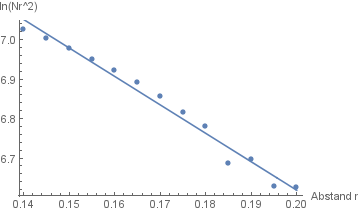
\includegraphics[width=0.6\textwidth]{images/relaxation.png}
	\end{tabular}
	\caption{Ausgleichsgerade zur Bestimmung der Relaxationslänge $\lambda$}
    \label{fig:relaxationsGerade}
\end{figure}
Aus der Steigung folgt die Relaxationslänge:
\begin{equation*}
\lambda = \frac{1}{a} = \unit[0.13886]{m}
\end{equation*}

\subsubsection{Statistischer Fehler}
Den statistischen Fehler der Relaxationslänge $\sigma_{\lambda}$ erhalten wir aus der Beziehung Steigung $a$ - Relaxationslänge $\lambda$ mit $\lambda=\frac{1}{a}$ durch Fehlerfortpflanzung:
\begin{equation*}
\sigma_{\lambda}=\frac{1}{a^2}\sigma_a=\unit[0.0060]{m}
\end{equation*}
\subsubsection{Systematischer Fehler}
Aus Gleichung \ref{eq:regressionRelaxation} folgt für die Relaxationslänge $\lambda$:
\begin{equation*}
\lambda=-\frac{r}{\ln{(Nr^2)} - c}
\end{equation*}
Mit Gaußscher Fehlerfortpflanzung erhalten wir den systematischen Fehler der Relaxationslänge:
\begin{align*}
\sigma_{\lambda}&=\sqrt{\left(\frac{\partial \lambda}{\partial r} \sigma_r\right)^2 + \left(\frac{\partial \lambda}{\partial N} \sigma_N\right)^2 + \left(\frac{\partial \lambda}{\partial c} \sigma_c\right)^2}\\
&=\sqrt{\frac{r^2\sigma^2_N + N^2(r^2 \sigma^2_c + (2+c)^2 \sigma^2_r)-2(2+c)N^2 \sigma^2_r \ln{(Nr^2)} + N^2 \sigma^2_r \ln{(Nr^2)}^2}{N^2(c-\ln{(Nr^2)})^4}}
\end{align*}
wobei $\sigma_c$ der Fehler des Konstanten $c$ aus dem obigen Fit ist:
\begin{align*}
\sigma_r&=\unit[0.0005]{m}\\
\sigma_c&=\unit[0.0535]{m^{-1}}\\
\sigma_N&=\sqrt{N}
\end{align*}
Für jedes gemessene Wertepaar kann nach obiger Vorschrift der systematische Fehler der Relaxationslänge berechnet werden. Einen Überblick erhält man in Tabelle \ref{tab:regressionRelaxationSysFehler}:
\begin{longtable}[H]{c|c|c}
$r$ $[m]$ & $N$ & $\sigma_{\lambda} [m]$\\
\hline
0.140 & \numprint{57418} & 0.211049\\
0.145 & \numprint{52315} & 0.202003\\
0.150 & \numprint{47584} & 0.192069\\
0.155 & \numprint{43379} & 0.182863\\
0.160 & \numprint{39859} & 0.174002\\
0.165 & \numprint{36092} & 0.164918\\
0.170 & \numprint{32833} & 0.155491\\
0.175 & \numprint{29730} & 0.145350\\
0.180 & \numprint{27176} & 0.137843\\
0.185 & \numprint{23391} & 0.119404\\
0.190 & \numprint{22398} & 0.121161\\
0.195 & \numprint{19866} & 0.109928\\
0.200 & \numprint{18850} & 0.109649\\
\caption{Systematische Fehler der Relaxationslänge $\sigma_{\lambda}$}
\label{tab:regressionRelaxationSysFehler}
\end{longtable}
Den systematischen Fehler der Relaxationslänge $\lambda$ erhalten wir aus dem Mittelwert der obigen Fehler mit $\unit[0.155825]{m}$. Als Endergebnis mit statistischem und systematischem Fehler bekommen wir:
\begin{equation*}
\boxed{\lambda=\unit[(0.1389 \pm 0.0060 \pm 0.1558)]{m}}
\end{equation*}
\subsection{Bestimmung der Diffusionslänge}
\label{subsec:diffusion}
Um die Diffusionslänge zu bestimmen, wird eine (punktförmige) Quelle für thermische Neutronen benötigt. Diese kann man auch durch eine Quelle schneller Neutronen erhalten, indem man, wie bereits erwähnt, die Zählraten einmal ohne Cadmium-Abschirmung und einmal mit Abschirmung des Detektors misst:
\begin{equation*}
N_{diff}=N_{ohne}-N_{mit}
\end{equation*}
Die Diffusionslänge erhält man aus Gleichung \ref{eq:flussThermisch}:
\begin{equation*}
\Phi(r)=\frac{Q}{4 \pi D} \cdot \frac{e^{-\frac{r}{L}}}{r}
\end{equation*}
Für den Fluss thermischer Neutronen gilt ausserdem:
\begin{equation*}
\Phi=\frac{N_{diff}}{t \cdot A}=\frac{N_{ohne}-N_{mit}}{t \cdot A}
\end{equation*}
Durch Gleichsetzen und Logarithmieren, ähnlich wie bei der Relaxationslänge, erhält man:
\begin{align}
\frac{N_{ohne}-N_{mit}}{t \cdot A}&=\frac{Q}{4 \pi D} \cdot \frac{e^{-\frac{r}{L}}}{r}\nonumber\\
\ln{((N_{ohne}-N_{mit}) \cdot r)}-\ln{(t \cdot A)}&=\frac{r}{L}+\ln{\frac{Q}{4 \pi D}}\nonumber\\
\ln{((N_{ohne}-N_{mit}) \cdot r)}&=\frac{r}{L} + const\label{eq:regressionDiffusion}
\end{align}
Die Diffusionslänge $L$ erhalten wir aus dem Kehrwert der Steigung der aus den $r$-, $\ln{((N_{ohne}-N_{mit}) \cdot r)}$-Wertepaaren gefitteten Gerade (siehe Tabelle \ref{tab:regressionDiffusion}).
\begin{longtable}[H]{c|c}
$r$ $[m]$ & $y=\ln{((N_{ohne}-N_{mit}) r)}$ $[m]$\\
\hline
0.140 & 4.94264\\
0.145 & 4.83286 \\
0.150 & 5.55933\\
0.155 & 5.07007\\
0.160 & 4.58088\\
0.165 & 4.36989\\
0.170 & 4.10858\\
0.175 & 4.24850\\
0.180 & 2.42834\\
0.185 & 5.46095\\
0.190 & 4.47915\\
0.195 & 4.91632\\
\caption{Punkte der Regressionsgerade zur Bestimmung der Diffusionslänge $L$}
\label{tab:regressionDiffusion}
\end{longtable}
Die Messung für den Abstand $\unit[20]{cm}$ lassen wir unberücksichtigt, weil dabei die Zählrate mit Cd-Abschirmung größer war als ohne (vgl. Tabelle \ref{tab:measurements}).
Der lineare Fit in Mathematica lieferte diese Ergebnisse:
\begin{eqnarray*}
a=\frac{1}{L}=-13.0271 \quad \quad \sigma_a=13.6829\\
c=6.76516 \quad \quad \sigma_c=2.30402
\end{eqnarray*}
Aus der Steigung erhalten wir die Diffusionslänge $L$:
\begin{equation*}
L=\unit[0.076763]{m}
\end{equation*}
\begin{figure}[H]
	\centering
	\begin{tabular}{@{}r@{}}
		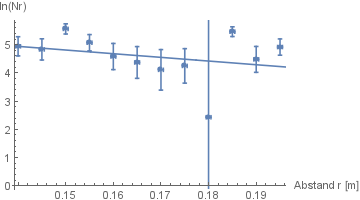
\includegraphics[width=0.8\textwidth]{images/diffusion.png}
	\end{tabular}
	\caption{Ausgleichsgerade zur Bestimmung der Diffusionslänge $L$}
    \label{fig:diffusionsGerade}
\end{figure}
Abbildung \ref{fig:diffusionsGerade} zeigt die Messdaten samt Fehlerbalken und die gefittete Gerade.

Dabei gelten für die $x$- und $y$-Achsen folgende Unsicherheiten:
\begin{description}
\item[$x$-Achse: Abstand $r$] \hfill \\
\begin{equation*}
\sigma_x=\sigma_r= \unit[0.0005]{m}
\end{equation*}
\item[$y$-Achse: der Ausdruck $\ln{((N_{ohne}-N_{mit}) \cdot r)}$] \hfill \\ Zunächst bestimmen wir die Unsicherheit $\sigma_{N_{diff}}$ von $N_{diff}=N_{ohne}-N_{mit}$. $N_{ohne}$ und $N_{mit}$ korrelieren nicht, weshalb wir die Gaußsche Fehlerfortpflanzung anwenden:
\begin{eqnarray*}
\sigma_{N_{diff}}&=&\sqrt{\left(\frac{\partial N_{diff}}{\partial N_{ohne}}\right)^2 \sigma^2_{N_{ohne}}+\left(\frac{\partial N_{diff}}{\partial N_{mit}}\right)^2 \sigma^2_{N_{mit}}}\\
&=&\sqrt{N_{ohne}+N_{mit}}
\end{eqnarray*}
Auch $N_{diff}$ und $r$ korrelieren nicht, also bestimmen wir die Unsicherheit $\sigma_y$ wieder mit der Gaußschen Fehlerfortpflanzung:
\begin{eqnarray*}
\sigma_y&=&\sqrt{\left( \frac{\partial y}{\partial N_{diff}} \right)^2 \sigma_{N^2_{diff}} + \left(\frac{\partial y}{\partial r}\right)^2 \sigma_{r^2}}\\
&=& \sqrt{ \left( \frac{r}{N_{diff}r}\right)^2 \cdot (N_{ohne}+N_{mit}) + \left(\frac{N_{diff}}{N_{diff} r}\right)^2 \sigma_r^2}\\
&=&\sqrt{\frac{N_{ohne}+N_{mit}}{(N_{ohne}-N_{mit})^2}+\frac{1}{r^2} \sigma_r^2}
\end{eqnarray*}
\end{description}
\subsubsection{Statistischer Fehler}
Analog zur Relaxationslänge lässt sich der statistische Fehler auf die Diffusionslänge aus der Beziehung Steigung-Diffusionslänge bestimmen:
\begin{equation*}
\sigma_L=\frac{1}{a^2}\sigma_a=\unit[0.0806274]{m}
\end{equation*}
\subsubsection{Systematischer Fehler}
Aus Gleichung \ref{eq:regressionDiffusion} folgt für die Diffusionslänge $L$:
\begin{equation*}
L=-\frac{r}{\ln((N_{ohne}-N_{mit}) \cdot r)-c}
\end{equation*}
Durch Fehlerfortpflanzung erhalten wir den systematischen Fehler der Diffusionslänge $\sigma_L$:
\begin{align*}
\sigma_L&=\sqrt{\left(\frac{\partial L}{\partial r} \sigma_r\right)^2 + \left(\frac{\partial L}{\partial N_{mit} }\sigma_{N_{mit}}\right)^2+\left(\frac{\partial L}{\partial N_{ohne}}\sigma_{N_{ohne}}\right)^2+\left(\frac{\partial L}{\partial c} \sigma_c\right)^2}\\
&=\sqrt{\frac{r^2 \sigma^2_c+\frac{r^2 \sigma^2_{N_{mit}}}{(N_{mit}-N_{ohne})^2} + \frac{r^2 \sigma^2_{N_{ohne}}}{(N_{mit}-N_{ohne})^2} + \sigma^2_r (1+c-\ln{((N_{ohne}-N_{mit})r})^2}{(c-\ln{((N_{ohne}-N_{mit}) r)})^4}}
\end{align*}
mit:
\begin{align*}
\sigma_r&=\unit[0.0005]{m}\\
\sigma_c&=\unit[2.30402]{m^{-1}}\\
\sigma_{N_{mit}}&=\sqrt{N_{mit}}\\
\sigma_{N_{ohne}}&=\sqrt{N_{ohne}}
\end{align*}
\newpage
Tabelle \ref{tab:regressionDiffusionSysFehler} zeigt die systematischen Fehler der Diffusionslänge für jeden Wertepaar.
\begin{longtable}[H]{c|c|c|c}
$r$ $[m]$ & $N_{mit}$ & $N_{ohne}$ & $\sigma_{\lambda} [m]$\\
\hline
0.140 & \numprint{57418} & \numprint{58419} & 0.098161\\
0.145 & \numprint{52315} & \numprint{53181} & 0.090652\\
0.150 & \numprint{47584} & \numprint{49315} & 0.238406\\
0.155 & \numprint{43379} & \numprint{44406} & 0.125257\\
0.160 & \numprint{39859} & \numprint{40199} & 0.078810\\
0.165 & \numprint{36092} & \numprint{36571} & 0.068209\\
0.170 & \numprint{32833} & \numprint{33191} & 0.058129\\
0.175 & \numprint{29730} & \numprint{30130} & 0.065866\\
0.180 & \numprint{27176} & \numprint{27239} & 0.041737\\
0.185 & \numprint{23391} & \numprint{24663} & 0.251284\\
0.190 & \numprint{22398} & \numprint{22862} & 0.085411\\
0.195 & \numprint{19866} & \numprint{20566} & 0.132455\\
\caption{Systematische Fehler der Diffusionslänge $\sigma_{\lambda}$}
\label{tab:regressionDiffusionSysFehler}
\end{longtable}
Wie bei der Relaxationslänge bestimmen wir den systematischen Fehler aus dem Mittelwert der einzelnen Fehler und erhalten als Ergebnis $0.111198$. Die Diffusionslänge $L$ mit Angabe der statistischen und systematischen Fehler beträgt:
\begin{equation*}
\boxed{L=\unit[(0.0768 \pm 0.0806 \pm 0.1112)]{m}}
\end{equation*}
\subsection{Diskussion der Ergebnisse}
\label{subsec:conclusion}
Wir haben berechnet:
\begin{align*}
\lambda&=\unit[(0.1389 \pm 0.0060 \pm 0.1558)]{m}\\
L&=\unit[(0.0768 \pm 0.0806 \pm 0.1112)]{m}
\end{align*}
Die Werte der Relaxations- und Diffusionslänge liegen im erwarteten Bereich; dabei ist die Relaxationslänge $\lambda$ größer als die Relaxationslänge $L$, was physikalisch einen Sinn hat, denn die schnellen Neutronen aufgrund ihrer hohen Energie größere Strecken ohne Wechselwirkung zurücklegen als die thermischen (Wirkungsquerschnitt steigt mit sinkender Energie).\\ \\
Die Fehler sind relativ zu den Längen groß. Das lässt sich darauf zurückführen, dass es verschiedene Angriffspunkte für Fehler gibt:
\begin{itemize}
\item Die Einstellung des mit einer Cd-Abschirmung umgebenden Detektors beeinflusste die gemessenen Zählraten erheblich. Bereits kleinste Korrekturen der Einstellung bei gleichem Detektor-Quelle-Abstand führten zu großen Schwankungen der Zählraten. Es ist davon auszugehen, dass die Abschirmung schlecht auf dem Detektor lag.
\item Die Zerfallsrate und folglich die gemessenen Zählraten unterliegen einer Poisson-Verteilung. Eine längere Dauer der Messung würde die Fehler reduzieren.
\item Der Abstand des Zählrohrs von der Neutronquelle wurde anhand einer Schiene auf dem Wassertank gemessen, wobei das Zählrohr selbst nicht sichtbar war. Möglicherweise befand sich das Zählrohr nicht direkt unter der Aufhängung auf der Schiene.
\item Wir arbeiten unter idealiserten Annahmen, denn wir sind in der Theorie von einer punktförmigen Quelle ausgegangen.
\end{itemize}

\section{Änderungsprotokoll}
\begin{table}[H]
\centering
\begin{tabularx}{\textwidth}{| c | c | X |}
\hline
\textbf{Datum} & \textbf{Abschnitt} & \textbf{Details}\\
\hline
9. Dezember 2014 & - & 1. Fassung\\
\hline
5. Januar 2015 & \ref{subsec:relaxation}, \ref{subsec:diffusion} und \ref{subsec:conclusion} & Zur Bestimmung der Relaxationslänge wurden die Messdaten der Messungen mit Cd-Abschirmung verwendet (vorher hatten wir Daten aus der Messung ohne Cd-Abschirmung verwendet), Korrektur und Vervollständigung der Fehlerrechnung (mit systematischem und statistischem Fehler), Überarbeitung der Diskussion der Ergebnisse\\
\hline
\end{tabularx}
\end{table}
\bibliographystyle{acm}
\bibliography{literatur}

\end{document}